\nsection{Dynamic Programming}

\subsection{Steiner-tree DP}
\ncomment{$n$ nodes, $k$ terminal nodes, unite all terminal nodes doing a Steiner tree}
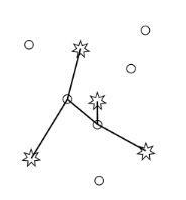
\includegraphics[width = 5cm]{../Codes/DynamicProgramming/SteinerTree.png}
\addfile{../Codes/DynamicProgramming/Steiner.cpp}
\vspace{-15pt}

\subsection{Matrix Chain Multiplication}
\addfile{../Codes/DynamicProgramming/MatrixChainMultiplication.cpp}

\subsection{Digit DP} 
\vspace{-5pt}
Counts the amount of numbers in $[l, r]$ such are divisible by $k$. (flag $nonzero$ is for different lengths)  \\
It can be reduced to $dp(i, x, small)$, and has to be solve like $f(r) - f(l - 1)$ \\
\vspace{-5pt}
\addfile{../Codes/DynamicProgramming/Digit.cpp}
\vspace{-15pt}

\subsection{Knapsack 0/1}
\addfile[5-7]{../Codes/DynamicProgramming/Knapsack01.cpp}

\subsection{Convex Hull Trick \complexity{n^2} $\Rightarrow$ \complexity{n}} 
\vspace{-15pt}
\begin{gather*}
dp[i] = \min_{j < i}(dp[j] + b[j] * a[i]) \\
dp[i][j] = \min_{k < j}(dp[i - 1][k] + b[k] * a[j]) \\
b[j] \geq b[j + 1] \text{ optionally } a[i] \leq a[i + 1] 
\end{gather*}
\vspace{-15pt}
\addfile[1-41]{../Codes/DynamicProgramming/ConvexHullTrick.cpp}

\subsection{Divide and conquer \complexity{kn^2} $\Rightarrow$ \complexity{k \cdot nlogn} } 
Split the array of size $n$ into $k$ continuous groups. $k \leq n$ \\
$cost(a, c) + cost(b, d) \leq cost(a, d) + cost(b, c)$ with $a \leq b \leq c \leq d$ \\
\addfile{../Codes/DynamicProgramming/DivideAndConquer.cpp}

\subsection{Do all submasks of a mask A}
\begin{code}
for (int B = A; B > 0; B = (B - 1) & A)
\end{code}

